Для того, чтобы повысить частоту сигнала, воспользуемся управлением непосредственно портами \textbf{ATmega}. Изменим в нашей программе строки

\begin{minted}[gobble=4,fontsize=\footnotesize]{c}
    digitalWrite(13, HIGH); //Turn on LED 13
    digitalWrite(13, LOW);  //Turn off LED 13
\end{minted}

на

\begin{minted}[gobble=4,fontsize=\footnotesize]{c}
    PORTB |= _BV(PORTB5);  //Turn on PORTB5
    PORTB &= ~_BV(PORTB5); //Turn off PORTB5
\end{minted}

PORTB5 является Pin 13 для Arduino UNO (ATmega328) и Pin 11 для Arduino MEGA 2560 (ATmega 2560). Диаграмма портов ATmega для Arduino представлена на рисунке~\ref{fig:a328diagram}.

\begin{figure}[ht]
    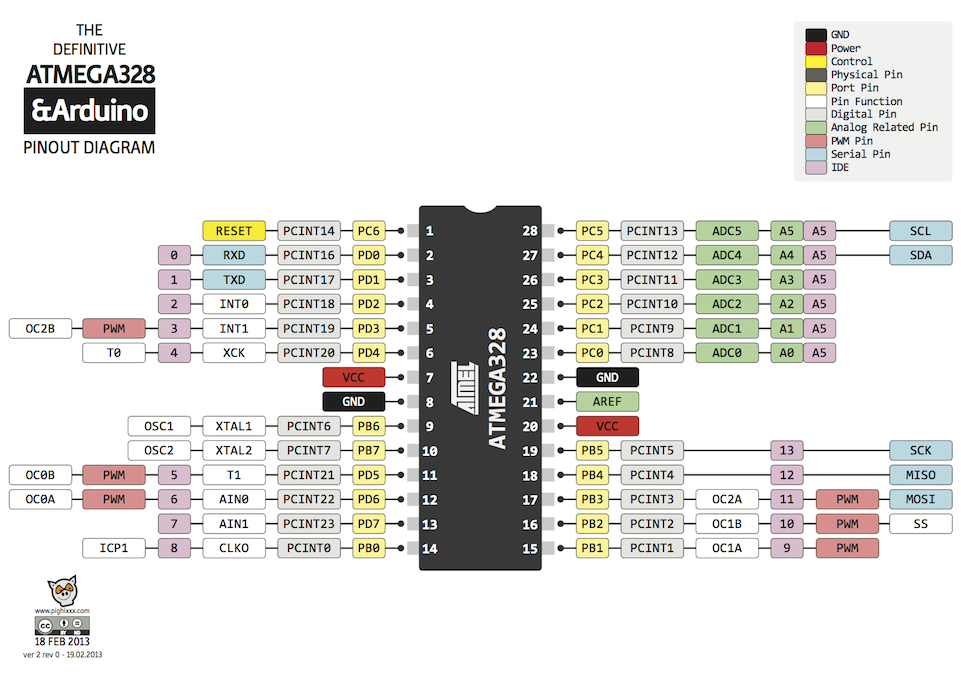
\includegraphics[width=1\linewidth]{Figures/a328diagram.png}
    \caption{Диаграмма портов ATmega328 для Arduino}
    \label{fig:a328diagram}
\end{figure}

В результате получаем значительный прирост скорости:

\begin{longtable}[c]{|c|c|}
    \caption{Результат работы напрямую с портами}
    \label{PortsResult}\\
    \hline
    \textbf{Количество, шт} & \textbf{Результат, мкс}\\
    \hline
    \endfirsthead
    \hline
    \textbf{Количество, шт} & \textbf{Результат, мкс}\\
    \hline
    \endhead
        1 & 6916\\
        \hline
        235 & 6940\\
        \hline
        328 & 6944\\
        \hline
        821 & 6948\\
        \hline
\end{longtable}

\begin{figure}[ht]
    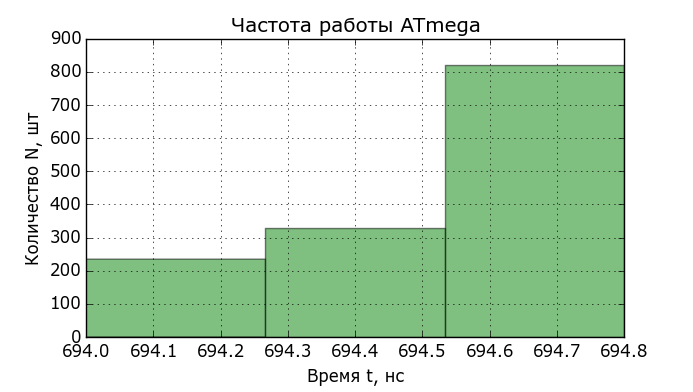
\includegraphics[width=.8\linewidth]{Figures/athist.png}
    \caption{Гистограмма измерений частоты ATmega}
    \label{fig:athist}
\end{figure}

То есть за счёт использования более низкого уровня взаимодействия с железом, мы добились увеличения скорости в $\frac{145928}{6948} = 21$ раз!

В итоге, максимальная скорость сигнала равна

\begin{equation}
    \label{eq:freq2}
    f = \frac{n}{t} = \frac{10000}{6948 \cdot 10^{-6}} = 1439263~\textrm{Гц} = 1.44~\textrm{МГц}
\end{equation}
